%
%===============>>  ГРУППА 9-2 МОДУЛЬ 7  <<=============
%
\setmodule{7}

%BEGIN_FOLD % ====>>_____ Занятие 1 _____<<====
\begin{class}[number=1]
	\begin{listofex}
		\item В треугольнике \( ABC \) угол \( C \) равен \( 90 \) градусов, \( AC=6 \), \( AB=20 \). Найдите \( \sin B \).
		\item  В треугольнике \( ABC \) угол \( C \) равен \( 90 \) градусов, \( BC=9 \), \( AB=20 \). Найдите \( \cos B \).
		\item В треугольнике \( ABC \) угол \( C \) равен \( 90 \) градусов, \( BC=9 \), \( AC=27 \). Найдите \( \tg B \).
		\item Найдите:
		\begin{tasks}(1)
			\task \( \sin\alpha \) и \( \tg\alpha \), если \( \cos\alpha=\dfrac{1}{2} \)
			\task \( \cos\alpha \) и \( \tg\alpha \), если \( \sin\alpha=\dfrac{\sqrt{3}}{2} \)
		\end{tasks}
		\item В треугольнике \( ABC \) угол \( C \) прямой, \( BC=8 \), \( \sin A=0,4 \). Найдите \( AB \).
		\item В треугольнике \( ABC \) угол \( C \) прямой, \( AC=15 \), \( \cos A=\dfrac{5}{7} \). Найдите \( AB \).
		\item В треугольнике \( ABC \) угол \( C \) равен \( 90\degree \), \( BC=12 \), \( \sin A=\dfrac{4}{11} \). Найдите \( AB \).
		\item Катеты прямоугольного треугольника равны \( \sqrt{15} \) и \( 1 \). Найдите синус наименьшего угла этого треугольника.
		\item Площадь прямоугольного треугольника равна \( 32\sqrt{3} \). Один из острых углов равен \( 30\degree \). Найдите длину гипотенузы.
		\item В треугольнике \( ABC \) угол \( C \) равен \( 90\degree \), \( AC=12 \), \( \tg A=\dfrac{2\sqrt{10}}{3} \).  Найдите \( AB \).
		\item В треугольнике \( ABC \) угол \( C \) равен \( 90\degree \), \( \sin A=\dfrac{4}{5} \), \( AC=9 \). Найдите \( AB \).
		\item Найдите синус меньшего острого угла между	диагональю прямоугольника и его стороной, если периметр прямоугольника равен \( 34 \) см, а одна из сторон --- \( 12 \) см. 
		\item Тангенс острого угла прямоугольного треугольника равен \( \dfrac{2}{5} \), а один из катетов на \( 6 \) см больше другого. Найдите площадь треугольника. 
		\item Основание равнобедренного треугольника равно \( 8 \) см, тангенс угла при основании равен \( 2 \). Найдите площадь треугольника. 
		\item Периметр равнобедренного треугольника равен \( 64 \) см, косинус угла при основании равен \( 0,6 \). Найдите площадь треугольника.
		\item В треугольнике \( ABC \) известно, что \( AB=8 \), \( BC=10 \), \( AC=12 \). Найдите \( \cos\angle ABC \).
		\item В треугольнике \( ABC \) сторона \( AB \) равна \( 2\sqrt{3} \), угол \( C \) равен \( 120\degree \). Найдите радиус описанной около этого треугольника окружности.
		\item Сторона правильного треугольника равна \( \sqrt{3} \). Найдите радиус окружности, описанной около этого треугольника.
		\item Найдите хорду, на которую опирается угол \( 120\degree \), вписанный в окружность радиуса \( \sqrt{3} \).  
		\item Сторона \( AB \) треугольника \( ABC \) равна \( 1 \). Противолежащий ей угол \( C \) равен \( 120\degree \). Найдите радиус окружности, описанной около этого треугольника.
		\item Угол \( C \) треугольника \( ABC \), вписанного в окружность радиуса \( 3 \), равен \( 30\degree \). Найдите сторону \( AB \) этого треугольника.
		\item Одна сторона остроугольного треугольника равна радиусу описанной около него окружности. Найдите угол треугольника, противолежащий этой стороне. Ответ дайте в градусах.
		\item В треугольнике \( ABC \) угол \( B \) равен \( 72\degree \), угол \( C \) равен \( 63\degree \), \( BC=2\sqrt{2} \). Найдите радиус описанной около этого треугольника окружности.
	\end{listofex}
\end{class}
%END_FOLD

%BEGIN_FOLD % ====>>_____ Занятие 2 _____<<====
\begin{class}[number=2]
	\begin{listofex}
		\item Выяснить вид треугольника (остроугольный, прямоугольный, тупоугольный), если длины его сторон равны \( 23 \) см, \( 17 \) см, \( 19 \) см. 
		\item Стороны треугольника равны \( 8\sqrt{3} \) см, \( \sqrt{577} \) см и \( \sqrt{11} \) см. Найдите наибольший угол	этого треугольника. 
		\item Две стороны параллелограмма равны \( 4 \) см и \( 5 \) см, а одна из диагоналей --- \( 46 \)
		см. Найти вторую диагональ параллелограмма.
		\item Боковая сторона равнобедренного треугольника равна \( 1 \), угол при вершине, противолежащей основанию, равен \( 120\degree \). Найдите диаметр описанной окружности этого треугольника.
		\item Радиус окружности, описанной около правильного треугольника, равен \( \sqrt{3} \). Найдите сторону этого треугольника.
		\item В треугольнике \( ABC \): \( \sin\angle B=0,6 \), \( AC=3 \), \( \angle C=30\degree \). Найдите \( AB \).
		\item Радиус окружности, описанной около треугольника \( ABC \), равен \( R \). Большая сторона треугольника \( ABC \) равна \( 10 \), а \( \angle ABC=150\degree \). Найдите \( R \).
		\item В треугольнике \( ABC \) проведена медиана \( AM \). Найдите площадь треугольника \( ABC \), если \( AC=3\sqrt{2} \), \( BC=10 \), \( \angle MAC=45\degree \).
		\item Площадь треугольника \( ABC \) равна \( 20\sqrt{3} \). Найдите \( AC \), если сторона \( AB \) равна \( 8 \), а медиана \( BM \) равна \( 5 \).
		\item В треугольнике \( ABC \): \( \angle A=45\degree \), \( O \) --- точка пересечения серединных перпендикуляров к сторонам \( AB \) и \( BC \), \( OD=44 \) --- серединный перпендикуляр к стороне \( CB \). Найдите \( CB \).
		\item Найдите угол \( ABC \), изображенный на рисунке. Ответ дайте в градусах.
		\begin{center}
			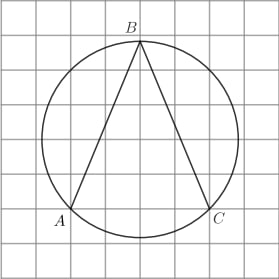
\includegraphics[align=t, width=0.3\linewidth]{\picpath/G92M7L2}
		\end{center}
		\item Найдите градусную меру дуги \( AC \) окружности, на которую опирается угол \( ABC \). Ответ
		дайте в градусах.
		\begin{center}
			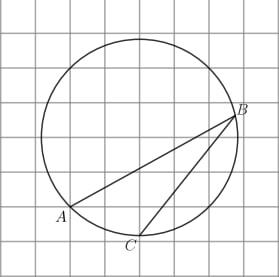
\includegraphics[align=t, width=0.3\linewidth]{\picpath/G92M7L2-2}
		\end{center}
		\item Найдите угол \( AOB \), изображенный на рисунке. Ответ дайте в градусах.
		\begin{center}
			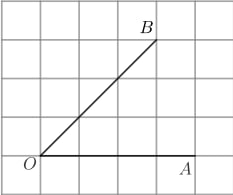
\includegraphics[align=t, width=0.3\linewidth]{\picpath/G92M7L2-3}
		\end{center}
		\item На клетчатой бумаге с размером клетки \( 1X1 \) изображён угол \( AOB \). Найдите его тангенс.
		\begin{center}
			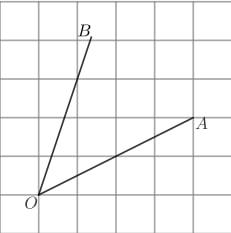
\includegraphics[align=t, width=0.3\linewidth]{\picpath/G92M7L2-4}
		\end{center}
	\end{listofex}
\end{class}
%END_FOLD

%BEGIN_FOLD % ====>>_ Домашняя работа 1 _<<====
\begin{homework}[number=1]
	\begin{listofex}
		\item В треугольнике \( ABC \) угол \( C \) равен \( 90\degree \), \( AC=9 \), \( AB=25 \). Найдите \( \sin B \).
		\item В треугольнике \( ABC \) угол \( C \) равен \( 90\degree \), BC\( =4 \), \( AC=28 \). Найдите \( \tg B \).
		\item В треугольнике \( ABC \) угол \( C \) равен \( 90\degree \), \( \sin B=\dfrac{5}{17} \), \( AB=51 \). Найдите \( AC \).
		\item В треугольнике\( ABC \) угол \( C \) равен \( 90\degree \), \( \tg B=\dfrac{8}{5} \), \( BC=20 \). Найдите \( AC \).
		\item Синус острого угла \( A \) треугольника \( ABC \) равен \( \dfrac{2\sqrt{6}}{5} \). Найдите \( \cos A \).
		\item В треугольнике \( ABC \) известно, что \( AB=6 \), \( BC=7 \), \( AC=8 \). Найдите \( \cos\angle ABC \).
		\item В треугольнике \( ABC \) угол \( A \) равен \( 60\degree \), угол \( B \) равен \( 45\degree \), \( BC=5\sqrt{6} \). Найдите \( AC \).
		\item Сторона правильного треугольника равна \( 3 \). Найдите радиус окружности, описанной около этого треугольника.
		\item В треугольнике \( ABC \) угол \( B \) равен \( 56\degree \), угол \( C \) равен \( 64\degree \), \( BC=3\sqrt{3} \). Найдите радиус описанной около этого треугольника окружности.
	\end{listofex}
\end{homework}
%END_FOLD

%BEGIN_FOLD % ====>>_____ Занятие 3 _____<<====
\begin{class}[number=3]
	\begin{listofex}
		\item Постройте график функции \( y=\dfrac{2x+1}{2x^2+x} \) и определите, при каких значениях \( k \) прямая \( y=kx \) имеет с графиком ровно одну общую точку.
		\item Постройте график функции \( y=\dfrac{1-2x}{2x^2-x} \) и определите, при каких значениях \( k \) прямая \( y=kx \) имеет с графиком ровно одну общую точку.
		\item Постройте график функции \( y=3-\dfrac{x+5}{x^2+5x} \) и определите, при каких значениях \( m \) прямая \( y=m \) не имеет с графиком ни одной общей точки.
		\item Прямая \( y=2x+b \) касается окружности \( x^2+y^2=5 \) в точке с положительной абсциссой. Определите координаты точки касания.
		\item Постройте график функции \( y=-4-\dfrac{x^4-x^3}{x^2-x} \) и определите, при каких значениях \( m \) прямая \( y=m \) имеет с графиком ровно две общие точки.
	\end{listofex}
\end{class}
%END_FOLD

%BEGIN_FOLD % ====>>_____ Занятие 4 _____<<====
\begin{class}[number=4]
	\begin{listofex}
		\item Постройте график функции
		\[y=	 \left\{
		\begin{array}{l}
			2x-2, \quad x<3\\
			-3x+13 \quad 3\leq x\leq4\\
			1,5x-7, \quad x>4.
		\end{array}
		\right. \]
		Определите, при каких значениях \( m \) прямая \( y=m \) имеет с графиком ровно две общие точки.
		\item Постройте график функции
		\[y=	 \left\{
		\begin{array}{l}
			x^2, \quad |x|\leq1\\
			-\dfrac{1}{x}, \quad |x|>1.
		\end{array}
		\right. \]
		При каких значениях параметра \( c \) прямая \( y=c \) имеет с графиком ровно одну общую точку.
		\item Постройте график функции
		\[y=	 \left\{
		\begin{array}{l}
			-x^2-4x-4, \quad x<-1\\
			1-|x-1|, \quad x\geq-1.
		\end{array}
		\right. \]
		При каких значениях параметра \( c \) прямая \( y=c \) имеет с графиком ровно две общие точки.
		\item При каких значениях \( m \) вершины парабол \( y =-x^2-6mx+m \) и \( y= x^2-4mx-2 \) расположены по одну сторону от оси \( x \)?		
		\item При каких значениях \( p \) вершины парабол \( y= -x^2+2px+3 \) и\( y= x^2-6px+p \) расположены по разные стороны от оси \( x \)?
		\item При каких значениях \( m \) вершины парабол \( y= x^2-4mx+m \) и \(y=-x^2+8mx+4 \) расположены по одну сторону от оси \( x \)?
	\end{listofex}
\end{class}
%END_FOLD

%BEGIN_FOLD % ====>>_ Домашняя работа 2 _<<====
\begin{homework}[number=2]
	\begin{listofex}
		\item Упростите выражение: \[ \left( \dfrac{4}{a+1}+\dfrac{2a}{a^2-1}+\dfrac{-1}{a-1} \right)\cdot(a^2+2a+1) \]
		\item При каких значениях \( m \) вершины парабол \( y=x^2+4mx+2m \) и \( y=-x^2+2mx+4 \) расположены по одну сторону от оси \( x \)?
		\item Постройте график функции
		\[y=	 \left\{
		\begin{array}{l}
			x^2+2x+3, \quad x\leq-3,\\
			x+9, \quad x>-3
		\end{array}
		\right. \]
		и определите, при каких значениях \( m \) прямая \( y=m \) имеет с графиком ровно две общие точки.
	\end{listofex}
\end{homework}
%END_FOLD

%BEGIN_FOLD % ====>>_____ Занятие 5 _____<<====
\begin{class}[number=5]
	\begin{listofex}
		\item Постройте график функции \( y=\dfrac{(\sqrt{x^2-5x+6})^2}{x-3} \) и найдите все значения \( a \), при которых прямая \( y=a \) не имеет с графиком данной функции общих точек.
		\item Постройте график функции \( y=\dfrac{x-2}{(\sqrt{x^2-2x})^2} \) и найдите все значение \( k \), при которых прямая \( y=kx \) имеет с графиком данной функции ровно одну общую точку.
		\item Постройте график функции \( y=x^2-3|x|-x \) и определите, при каких значениях \( c \) прямая \( y=c \) имеет с графиком три общие точки.
		\item Постройте график функции \( y=|x-2|-|x+1|+x-2 \) и найдите значения \( m \), при которых прямая \( y=m \) имеет с ним ровно две общие точки.
		\item Постройте график функции \( y=\dfrac{|x|-4}{x^2-4|x|} \) и определите, при каких значениях \( k \) прямая \( y=kx \) не будет иметь с построенным графиком ни одной общей точки.
		\item Постройте график функции \( y=|x-3|-|x+3| \) и найдите все значения \( k \), при которых прямая \( y=kx \) имеет с графиком данной функции ровно одну общую точку.
	\end{listofex}
\end{class}
%END_FOLD

%BEGIN_FOLD % ====>>_____ Занятие 6 _____<<====
\begin{class}[number=6]
	\begin{listofex}
		\item Первая прямая проходит через точки \( (0; 4,5) \) и \( (3; 6) \). Вторая прямая проходит через точки \( (1;2) \) и \( (-4;7) \). Найдите координаты общей точки этих двух прямых.
		\item Прямая \( y=2x+b \) касается окружности \( x^2+y^2=5 \) в точке с положительной абсциссой. Определите координаты точки касания.
		\item Найдите наименьшее значение выражения \( (5x-4y+3)^2+(3x-y-1)^2 \) и значения \( x \) и \( y \), при которых оно достигается.
		\item Найдите наименьшее значение выражения и значения \( x \) и \( y \), при которых оно достигается \( |6x+5y+7|+|2x+3y+1| \).
		\item Найдите наибольшее значение выражения \( \dfrac{x^3-y}{x^2+1}-\dfrac{x^2y-x}{x^2+1} \),  если \( x \) и \( y \) связаны соотношением \( y=x^2+x-4 \).
		\item Найдите все значения \( a \), при которых неравенство \( x^2+(2a+4)+8a+1\le0 \) не имеет решений.
	\end{listofex}
\end{class}
%END_FOLD

%BEGIN_FOLD % ====>>_ Домашняя работа 3 _<<====
\begin{homework}[number=3]
	\begin{listofex}
		\item Постройте график функции \( y=\dfrac{(\sqrt{x^2+3x})^2}{x} \).  Найдите значения \( a \), при которых прямая \( y=a \) не имеет с графиком данной функции общих точек.
		\item Постройте график функции \( y=|x-1|-|x+1| \) и найдите все значения \( k \), при которых прямая \( y=kx \) имеет с графиком данной функции ровно одну общую точку.
		\item Найдите наименьшее значение выражения и значения \( x \) и \( y \), при которых оно достигается \( |3x-4y-2|+|x-5y+3| \).
	\end{listofex}
\end{homework}
%END_FOLD

%BEGIN_FOLD % ====>>_____ Занятие 7 _____<<====
\begin{class}[number=7]
	%\title{Подготовка к проверочной}
	\begin{listofex}
		\item Постройте график функции \(y=\dfrac{ x^4-13x^2+36 }{ (x-3)(x-2) }\) и определите,при каких значениях параметра \(c\) прямая \(y=c\) имеет с графиком ровно одну общую точку.
		\item При каких значениях \(p\) вершины парабол \(y=-x^2+2px+3\) и \\ \(y=x^2-6px+p\) расположены по разные стороны от оси \(x\)?
		\item При каких значениях \(m\) вершины парабол \(y=-x^2-6mx+m\) и \\ \(y=x^2-4mx-2\) расположены по одну сторону от оси \(x\)?
		\item Постройте график функции \[ y= \begin{cases} -x^2-4x-4, \quad x<-1 \\ 1-|x-1|, \quad x\ge-1 \end{cases} \] и определите, при каких значениях параметра \(a\) он имеет ровно две общие точки с прямой \(y=a\).
		\item Постройте график функции \( y=\dfrac{ 1 }{ 2 }\left( \left| \dfrac{ x }{ 3,5 }-\dfrac{ 3,5 }{ x } \right| +\dfrac{ x }{ 3,5 } + \dfrac{ 3,5 }{ x } \right) \) и определите, при каких значениях \(m\) прямая \(y=m\) имеет с графиком ровно одну общую точку.
	\end{listofex}
\end{class}
%END_FOLD

=%BEGIN_FOLD % ====>>_ Проверочная работа _<<====
\begin{exam}
	\begin{listofex}
		\item Проверочная
	\end{listofex}
\end{exam}
%END_FOLD